\section{Approach}
Plenty of literature exists on modeling both surface rail networks, which typically cover longer distances, and subway or light-rail systems, which typically operate with a higher train frequency. Where simulations of surface rail networks might focus on maintaining arrival and departure schedules, subway and metro systems are more interested in keeping the trains moving and avoiding deadlock.  Deadlock is a state where no train can advance.  For example, consider a scenario where a train is broken down for an extended period of time.  As time advances, trains continue to arrive behind the disabled train, but are unable to pass.  Eventually all trains are stuck behind the disabled train.  Careful placement and management of track switches can be used to allow trains to overtake and pass a disabled train. These management schemes require modeling and simulation to evaluate their effectiveness.  According to Ref.~\citen{ttcservice}, Toronto subway trains run every two to seven minutes. Even small delays of just a couple minutes can result in relatively significant delays.

The approach considered here consists of five atomic components coupled together: stations, track sections, trains, passengers and a scheduler. A hierarchy and some simple relationships between the components are shown in Fig.~\ref{fig:hierarchy}.  Stations and track sections are modeled similarly, with the exception that passengers can be unloaded and loaded at stations. A subway line is modeled as a continuous loop. For example, a subway line with two endpoints is modeled as one continuous loop by having instances of stations for each direction--east and west, for example. In this setup, each stop has two station instances: a west station and an east station.  At one endpoint where the east station is reached, the west station is the very next station in the loop and vice versa for the other end point.  Each train carries up to a specified maximum number of passengers. The time to load and unload passengers is specified as some minimum value, plus an optional random component. Passengers originate and terminate at stations.  Trains may also suffer from failures, which cause delays in service.  The primary role of the scheduler is to control the movement of the trains and ensure no collisions or deadlocks occur.  The models for these components are described in more detail in the following sections.
%
\begin{figure}[htb]
	\centering
	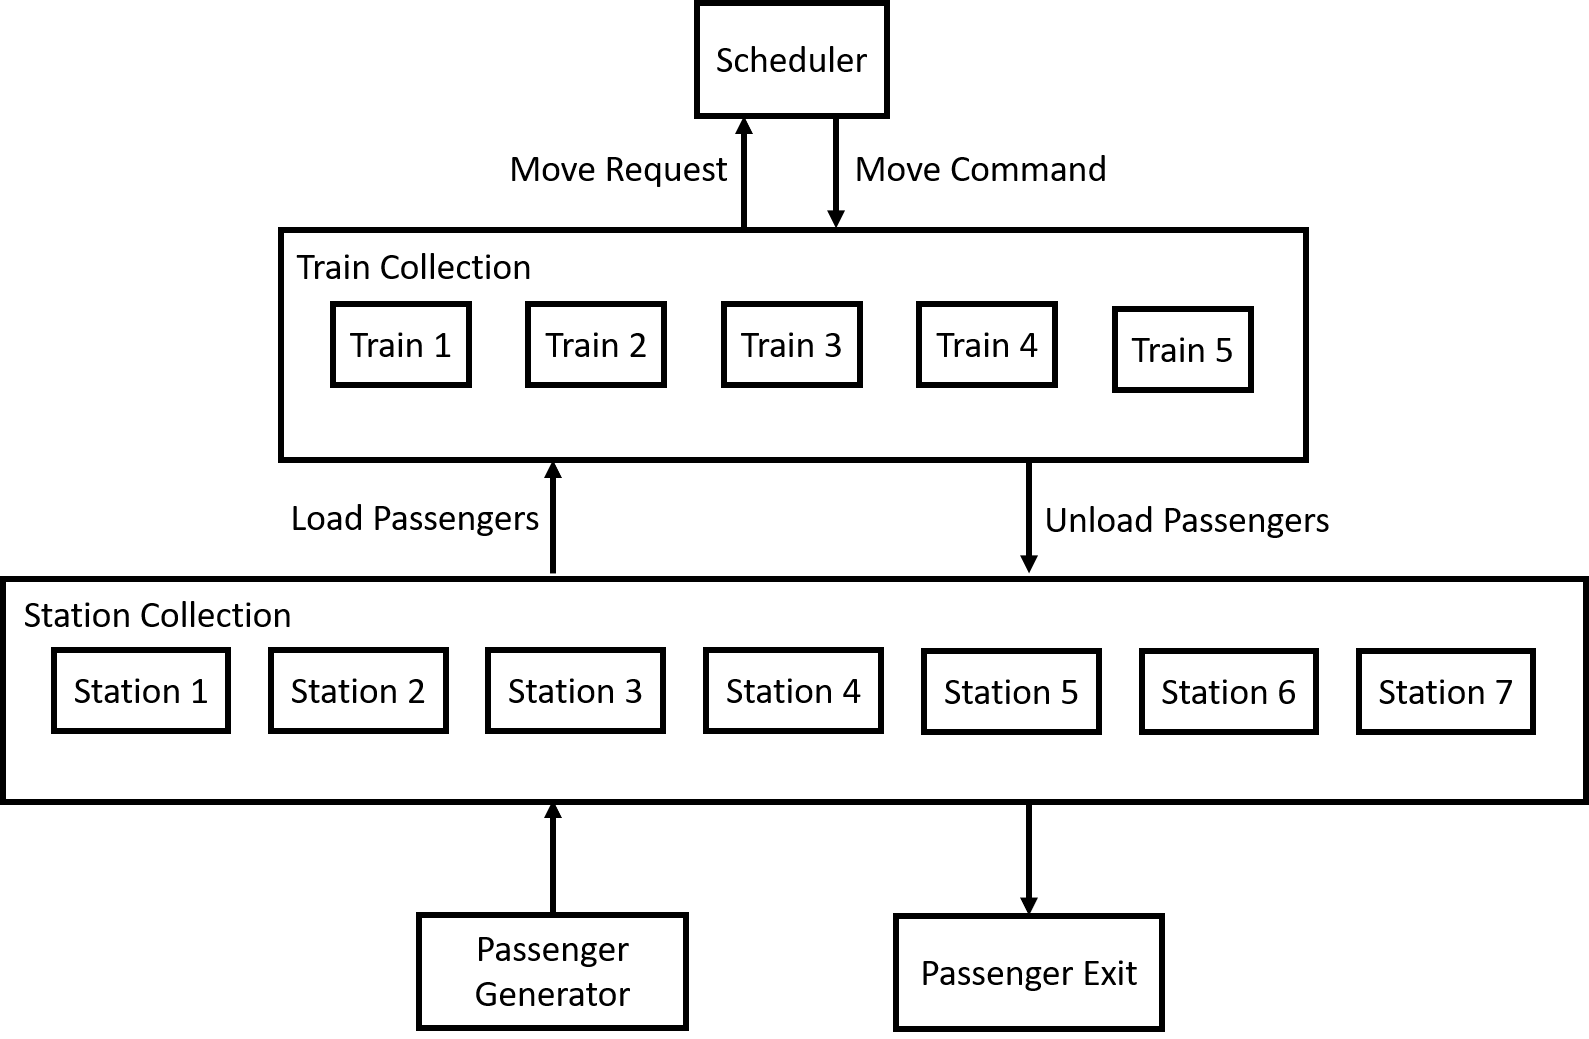
\includegraphics[width=6.5in]{hierarchy.png}
	\caption{Component Hierarchy}
	\label{fig:hierarchy}
\end{figure}
%
\subsection{Time Advance Scheme}
All of the models discussed in the following sections, with the exception of the train model, operate in zero time.  None of their state transitions result in any time advance.  Instead, all time advancement is computed in the train instances. While stations handle production and disposal of passengers, they yield no advancement in time to perform these functions.  The train will advance time when boarding or unloading passengers and traveling across track sections.
%
\subsection{Station Model}
The station serves as the creation and destruction point for passengers.  The station is also the only location where trains may load or unload passengers. The station is responsible for maintaining a pool of waiting passengers.  If a train does not have enough capacity to board all waiting passengers, then those passengers persist at the station and wait for the next train.  Also, if at any point a train must unload all of its passengers, in the event of an extended breakdown for example, any passengers not at their final destination will be added to the waiting passengers queue. In generating passengers, the station implements multiple options for generating destinations for each passenger.  In each of the destination options, the destinations are chosen from a predefined set of destinations that does not include the origin station.  One method for generating the destination is to loop through the possible destinations repeatedly, in order.  Another method is to specify a single destination for all passengers.  The third option is to generate a random destination.

The inputs to the station are a set of passengers to unload from the arriving train and the available capacity of the arriving train.  Both of these values are contained within the same message on the input port.  This accomplished with a new derived \texttt{Entity} type.  The output is a set of passengers to load onto the train. For its states, the station may be simply waiting, unloading passengers from a train, or providing passengers to a train.  The station model must also have a state variable that holds the current waiting passenger collection. 

After unloading passengers from a train, the station immediately updates its waiting passenger list.  The amount of passengers generated is specified by a rate.  The rate is given in units of passengers per minute.  When generating passengers, the total amount of passengers generated at that instant is the specified rate multiplied by a time.  The time used is the difference between the current internal clock value and the previous clock value at which passengers were created.  The internal clock and previous passenger generation time are both stored in state variables.  Once the created passengers are added to the waiting passengers list, the station takes up to as many passengers as the current train capacity from the front of the list adds them to a list of passengers to load on the train.  This list is then sent along with the unique station identifier as output.  The unique station identifier is used by the scheduler/coordinator to route the passengers to the correct train.  The scheduler is discussed in more detail in a later section. 
\begin{align*}
DEVS_{\textrm{Station}} &= \left<X,Y,S,\delta_{ext},\delta_{int},\lambda,ta\right> \\
P &= Passenger\ Collection, |P|\in\mathbb{N}_0^+ \\
P_w &= \text{Waiting passenger list} \\
P_l &= \text{List of passengers to load} \\
C &= \text{Passenger capacity of current train} \\
ID &= \text{Unique station identifier} \\
X &= \lbrace(\text{``Unload Passengers''},\lbrace P, C|C\in\mathbb{N}_0\rbrace)\rbrace \\
Y &= \lbrace(\text{``Load Passengers''},\lbrace P_l|\ |P_l|\leq C, P_l\subseteq P_w\rbrace\cup\emptyset)\rbrace \\
S_{clock} &= \mathbb{R}_0^+ \\ 
S_{timeOfLastPassengerCreation} &= \mathbb{R}_0^+ \\
S_{action} &= \lbrace\text{``passive'', ``Unload Passengers'',} \\
	& \text{``Load Passengers''}\rbrace \\
S_{waitingPassengers} &= \lbrace P_w, |P_w|\in\mathbb{N}_0^+\rbrace \\
S_{loadingPassengers} &= \lbrace P_l, |P_l|\leq C\rbrace \\ 
S &= S_{action}\times S_{clock}\times \\
 & S_{timeOfLastPassengerCreation}\times S_{waitingPassengers} \\
 & S_{loadingPassengers}\times \mathbb{R}_0^+ \\
\delta_{ext}(\text{``passive''},e,(\text{``Unload Passsengers''},\lbrace u|u\in\mathbb{N}_0\rbrace)) &= (\text{``Unload Passengers''},0,\lbrace P, C\rbrace) \\
\delta_{int}(\text{``passive''}) &= \text{``passive''} \\
\delta_{int}(\text{``Unload Passengers''},\sigma) &= (\text{``Load Passengers''},0,\lbrace ID, P\rbrace)\rbrace\ \\
\delta_{int}(\text{``Load Passengers''},\sigma) &= (\text{``passive''}) \\
\delta_{con}(s,ta(s),x) &= \delta_{ext}(\delta_{int}(s),0,x) \\
\lambda(\text{``Load Passengers''}) &= \lbrace ID,\lbrace P, |P|\leq C\rbrace\cup\emptyset\rbrace \\
ta(s) &= 0 \\
ta(``passive'') &= \infty \\
\end{align*}
%
\subsection{Track Section Model}

The track section model is needed to control access to track sections. A train
is permitted to enter a section if there is remaining capacity in the section.
When a train leaves a section the section's remaining capacity is increased by
one. Acquire and release requests are sorted by train ID so that the external
transition does is not determined by an arbitary bag ordering. The track 
section model can be represented by the DEVS with ports model below.

\newcommand{\InEnterReq}[0]{(\text{``Enter Request''}, \text{TrainID})}
\newcommand{\InExitReq}[1]{(\text{``Exit Request''}, \text{TrainID})}

\newcommand{\OutEnterRes}[1]{(\text{``Enter Response''}, #1)}

\begin{flalign*}
    &DEVS_{\textrm{Track}} = \left<X,Y,S,\delta_{ext},\delta_{int},\lambda,ta\right>& \\
    &A = \text{Number of trains allowed on section}& \\
    &X = \{ \InEnterReq, \InExitReq \} & \\
    &Y = \{\OutEnterRes{\{\text{May enter}, \text{May not enter}\}}\}& \\
    &Acquired = \text{Set of possible Train ID Sets}& \\
    &M = \text{Set of acquire and release messages}& \\
    &S = \{ (p, a, m, \sigma) | p \in \{passive, busy\}, a \in Acquired, a \leq A, \sigma \in \mathbb{R}_0^+ \}& \\
    &ta((\_, \_, \_, \sigma)) = \sigma& \\
    &\delta_{int}((p, a, m, \_)) = (passive, a, \{ \}, \infty)& \\
    \intertext{Input messages are split into acquires and releases and sorted by train ID} 
    &\delta_{ext}((p, a, m, \sigma), e, ((), ())) = (busy, a, m, 0)& \\
    &\delta_{ext}((p, a, m, \_), e, ((), acquires)) =& \\ 
    &\quad\begin{cases}
        \delta_{ext}((busy, a.add(head(acquire)), m.add((head(acquire), true)), 0), e, (tail(acquires), ())) \\ \quad\text{if\;} a > 0, head(acquires) \not\in a \\
        \delta_{ext}((busy, a, m.add((head(acquire), false)), 0), e, (tail(acquires), ())) \\ \quad\text{if\;} a > 0, head(acquires) \in a \\
    \end{cases}& \\
    &\delta_{ext}((p, a, m, \_), e, (releases, acquires)) =& \\ 
        &\quad\begin{cases}
            \delta_{ext}((busy, a.remove(head(releases)), m.add((head(releases), true)), 0), e, (tail(releases), (acquires))) \\ \quad\text{if\;} a > 0, head(releases) \in a \\
            \delta_{ext}((busy, a, m.add((head(releases), false)), 0), e, (tail(releases), (acquires))) \\ \quad\text{if\;} a > 0, head(releases) \not\in a \\
        \end{cases}& \\
    &\lambda((\_, \_, m, \_)) = m&
\end{flalign*}

\subsection{Subway Loop Model}

To simplify couplings between the large numbers of stations and tracks with the scheduler, the subway loop model is a digraph that contains the stations and tracks for a given subway line.  The subway loop model has the same input and output ports as the stations and tracks.  As the input and output ports for the subway loop model are coupled to every instance of a station or track section contained within, the station and track section models must filter the messages based on the unique identifier that is passed along with each message. Thus, all station instances receive all station messages and all track sections receive all track messages, but filtering the processing of the messages based on the unique identifier means only the targeted instance will process a given message. The subway loop model stores the stations and tracks in a circular array.  It is assumed that stations are located at even indices in the array and track sections at odd indices. This allows the scheduler to quickly identify whether a train is at a station or on a track section using just an integer array index value.

\subsection{Train Model}

Trains travel station to station to unload and load passengers. Sometimes they
break down. They also follow a movement protocol and a loading and unloading
protocol. In the loading and unloading protocol, a train arrives at a station,
unloads some of its passengers, waits for a capacity request, responds with a
remaining capacity and awaits for the station to load the train. In the movement
protocol, the train asks the scheduler if it can be move forward and scheduler
replies with an accepted or rejected. Trains rejected from proceeding to the
next section still proceed as far as they can within their section. This
behavior is represented by the DEVS with ports model below. Any missing
transitions are assumed to return the input state. 

The model makes some simplifying assumptions. It assumes that each track section
includes stations and the track up to the next station. This assumption could be
relaxed by having the train keep track of whether or not the train is at a
station. A 50\% disembark rate is also assumed for unloading at each station. A
more detailed model would include each passengers destination station so that
forced breakdowns event would force passengers to exit and those that did not
reach their desired destination would board the next train (this model assumes
disembarkers never reboard). It also assumes that breakdown repair times and in
need of repair times are constant.

\newcommand{\InBreakDown}[0]{(\text{``Breakdown''}, ())}
\newcommand{\InCapReq}[0]{(\text{``Capacity Request''}, ())}
\newcommand{\InMoveRes}[1]{(\text{``Move Response''}, #1)}
\newcommand{\InLoadPassengers}[1]{(\text{``Load Passengers''}, #1)}

\newcommand{\OutRemainingCapacity}[1]{(\text{``Remaining Capacity''}, #1)}
\newcommand{\OutUnloadPassengers}[1]{(\text{``Unload Passengers''}, #1)}
\newcommand{\OutMoveReq}[1]{(\text{``Move Request''}, #1)}
\newcommand{\phase}[0]{\text{phase}}

\newcommand{\Mod}[2]{\mathrm{mod} (#1, #2)}

\begin{align*}
DEVS_{\textrm{Train}} &= \left<X,Y,S,\delta_{ext},\delta_{int},\lambda,ta\right> \\
    T &= \text{\# of trains} \\
    N &= \# \text{\;of train stations} \\
    C &= \text{Passenger capacity of train} \\
    m &= \text{Travel time from end of track} \\
        & \text{section to next section} \\
    X &= \{
      \InBreakDown, \\
      &  \InCapReq, \\
      &  \InLoadPassengers{\{ p | p \in \mathbb{N}_0, p \leq C \}} \\
      &  \InMoveRes{\{ \text{Accepted}, \text{Rejected} \}}
    \} \\
    Y &= \{
      \OutRemainingCapacity{\{ c | c \in \mathbb{N}_0 \}}, \\
      &  \OutUnloadPassengers{\{ u | u \in \mathbb{N}_0 \}}, \\
      &  \OutMoveReq{\\ 
        & \{ (i, t) | i \in \mathbb{N}_0, i < N, t \in \mathbb{N}_0, t < T \}}
    \} \\
    S_{action} &= \{
      \text{moving}, \text{needs repairs}, \text{in repair}, \\
      &  \text{loading}, \text{unloading}, \text{waiting for load}, \\
      &  \text{waiting for cap req} 
    \} \\
    S_{\text{position}} &= \{ i | i \in \mathbb{N}_0, i < N
    \} \\
    S_{passengers} &= \{ p | p \in \mathbb{N}_0, p \leq C \} \\
    S &= S_{action} \times S_{position} \times S_{passengers} \times \sigma \\
    ta(a, i, p, \sigma) &= \sigma \\
    %
    \delta_{ext}((\text{moving}, i, p, \sigma), e, \InBreakDown) &= 
        (\text{needs repair}, i, p, \\
        & \text{time till repairs start}) \\
    \delta_{ext}((\text{moving}, i, p, \sigma), e, \InMoveRes{\text{Accepted}})
        &= (\text{unloading}, \Mod{i+1}{N}, \ceil*{p/2}, \\
        & \text{loading time}) \\
    \delta_{ext}((\text{moving}, i, p, \sigma), e, \InMoveRes{\text{Rejected}})
        &= (\text{moving}, i, p, \max(m, \sigma - e)) \\
    \delta_{ext}((\text{waiting for cap req}, i, p, \sigma), e, \InCapReq) &=
        (\text{waiting for load}, i, p, \infty) \\
    \delta_{ext}((\text{waiting for load}, i, p, \sigma), e, \InLoadPassengers{p_{load}}) &=
        (\text{loading}, i, p + p_{load}, \text{loading time}) \\
    %
    \delta_{int}(\text{unloading}, i, p, \sigma) &= 
        (\text{waiting for cap req}, i, p, \infty) \\
    \delta_{int}(\text{loading}, i, p, \sigma) &= (\text{moving}, i, p,
        \text{time to next station}) \\
    \delta_{int}(\text{needs repair}, i, p, \sigma) &= 
        (\text{in repair}, i, p, \text{repair time}) \\
    \delta_{int}(\text{in repair}, i, p, \sigma) &= 
        (\text{moving}, i, p, \text{time to next station}) \\
    %
    \lambda(\text{moving}, i, p, \sigma) &= \OutMoveReq{(i, t)} \\ 
        & \text{\;where\;} t \text{\;is the constant train ID} \\
    \lambda(\text{unloading}, i, p, \sigma) &= \OutUnloadPassengers{\floor*{p/2}} \\
    \lambda(\text{waiting for cap req}, i, p, \sigma) &= \OutRemainingCapacity{C - p}
\end{align*}
%
\subsection{Train Group Model}
Similar to the subway loop model, the train group model is used to simplify port coupling between the scheduler and all of the trains.  Messages sent from the scheduler to the train group are filtered by the train instances using a unique train identifier.  The order of the trains as stored in the train group model is unimportant.  The train group model contains the same input and output ports as the train model.

\subsection{Scheduler Model}
A formal definition of the scheduler model as implemented in the DEVS suite is provided below.  A scheduler is essentially a coordinator model, but since in this case its primary purpose is to maintain the subway train schedule, we identify it as the scheduler. It routes all message traffic between a group of trains and the subway loop, where the subway loop is composed of alternating station and track instances.  Without the scheduler to route messages from trains to the appropriate stations and vice versa, every train would need to be coupled to every track and every station.  Any time an output is sent from a train, it would be received by every track and every station instance as we are unable to rebind the train ports each time it moves to a new track or station. Instead, each time a train generates an output, it sends it only to the scheduler.  The scheduler will then identify to which station or track the message is targeted and repackage and send the message accordingly. Conversely, when a station needs to send a message to a train, the scheduler also manages the reverse association.  
%
\begin{align*} DEVS_{\textrm{Scheduler}} &= \left<X,Y,S,\delta_{ext},\delta_{int},\lambda,ta\right> \\
C &= \text{Remaining train capacity} \\
P &= \text{A list of passengers}\cup\emptyset \\
T &= \text{A group of trains} \\
L &= \text{A loop of track and station instances} \\
X &= \lbrace (\text{``Unload Passengers''},(Train\ ID, P, C)), \\
 & (\text{``Request Move to Station''},(Train\ ID)), \\
 & (\text{``Request Move to Track''},(Train\ ID)), \\
 & (\text{``Passengers to Load''},(Station\ ID, P)), \\
%& (\text{``Breakdown''},(Train\ ID,\mathbb{R}_0^+)), \\
 & (\text{``Acquire''},(x|x\in\lbrace True,False\rbrace)), \\
 & (\text{``Release''},(x|x\in\lbrace True,False\rbrace))\rbrace \\
Y &= \lbrace(\text{``Move to Track''},(Train\ ID,\mathbb{R}_0^+)), \\
 & (\text{``Move to Station''},(Train\ ID, Station\ ID)), \\
 & (\text{``Board Passengers''},(Train\ ID, P)), \\
 & (\text{``Unload Passengers''},(Station\ ID, P)), \\
 & (\text{``Acquire''},(Train\ ID)), \\
 & (\text{``Release''},(Train\ ID)), \\
 & (\text{``N Passengers Delivered''},(\mathbb{N}_0^+)) \\
S_{action} &= \lbrace \text{``passive'',``processing''}\rbrace \\
S_{trainPosition} &= \lbrace t_k|t_k\in\mathbb{N}_0^+, 0\leq k<|T|\rbrace \\
S_{segmentPopulated} &= \lbrace x_k|x_k\in\lbrace True,False\rbrace, 0\leq k<|L|\rbrace \\
S &= S_{action}\times S_{trainPosition}\times \\
 & S_{segmentPopulated}\times\mathbb{R}_0^+ \\
\delta_{ext}(\text{``passive''},e,(\text{``Unload Passengers''},&(Train\ ID,P,C))) = \\ &(\text{``processing''},0,(Train\ ID,P,C)) \\
\delta_{ext}(\text{``passive''},e,(\text{``Request Move to Station''},&(Train\ ID))) = \\
&(\text{``processing''},0,(Train\ ID)) \\
\delta_{ext}(\text{``passive''},e,(\text{``Request Move to Track''},&(Train\ ID))) = \\
&(\text{``processing''},0,(Train\ ID)) \\
\delta_{ext}(\text{``passive''},e,(\text{``Passengers to Load''},&(Station\ ID,P))) = \\
&(\text{``processing''},0,(Station\ ID)) \\
\delta_{ext}(\text{``passive''},e,(\text{``Acquire''},&(boolean))) = \\
&(\text{``processing''},0,(boolean)) \\
\delta_{ext}(\text{``passive''},e,(\text{``Release''},&(boolean))) = \\
&(\text{``processing''},0,(boolean)) \\
\delta_{int}(\text{``processing''},\sigma) &= \text{``passive''} \\
\delta_{int}(\text{``passive''}) &= \text{``passive''} \\
\delta_{con}(s,ta(s),x) &= \delta_{ext}(\delta_{int}(s),0,x) \\
\lambda(\text{``Move to Track''},\sigma,(Train\ ID,\mathbb{R}_0^+)) &= (\text{``Move to Track''},T\times\mathbb{R}_0^+) \\
\lambda(\text{``Move to Station''},\sigma,(Train\ ID,Station\ ID)) &= (\text{``Move to Station''},T\times S | S\subset L) \\
\lambda(\text{``Board Passengers''},\sigma,(Train\ ID,P)) &= (\text{``Board Passengers''},T\times P) \\
\lambda(\text{``Unload Passengers''},\sigma,(Station\ ID,P)) &= (\text{``Unload Passengers''}, S\times P | S\subset L) \\
\lambda(\text{``Acquire''},\sigma,(Train\ ID)) &= (\text{``Acquire''},t\in T) \\
\lambda(\text{``Release''},\sigma,(Train\ ID)) &= (\text{``Release''},t\in T) \\
\lambda(\text{``N Passengers Delivered''},\sigma,(\mathbb{N}_0^+)) &= (\text{``N Passengers Delivered''},n\in \mathbb{N}_0^+) \\
ta(s) &= 0 \\ 
ta(\text{``passive''}) &= \infty \\
\end{align*}

Note that the current implementation of the scheduler does not actually make use of the \textit{Acquire} and \textit{Release} features of the track section models. These semaphores are key in facilitating coupling in a simulation of multiple subway lines.  The intent is that multiple lines might share sections of track.  The semaphores are then necessary to ensure that only a specified number of trains are on a section of track at a time.  This is particularly useful when considering a pass capability.  If one train is blocking a section of track, using switches it would be possible for trains to bypass the blockage by temporarily switching over to the other side of the track. Because track instances can be shared by reference across multiple subway lines, the semaphores are needed to ensure a path around a blockage is available.  However, even though the basic framework exists for implementing this logic, given time constraints this logic was unable to be fully completed.
\subsubsection{Scheduler Logic}
The scheduler is the logic center of the simulation. Any train movement decisions are made exclusively by the scheduler. Since the trains are not directly coupled to the stations and track sections, the trains have no immediate knowledge of where they are, nor are they able to inquire. The scheduler uses a HashMap to map train IDs to an integer value which represents an index on the subway loop circular list.  This index defines the train position.  To move a train, the index is incremented. A boolean array stores which sections of the subway loop are occupied. This boolean array is also modified each time a train is moved to ensure the scheduler is able to quickly check for collisions.  The track section semaphores, once fully implemented, would take the place of this boolean array as a much more robust collision detection method. The boolean array method does not currently allow for one train to pass another in the same direction of travel.
\begin{equation}
x_{n+1} = (x_n+1)\mod L
\end{equation}
where $x_{n+1}$ is the next position, $x_n$ is the current position, and $L$ is the total number of stations and track segments in the subway loop.  This gives an effective circular array. It is the user's responsibility to ensure that the last element in the subway loop should be a segment that is physically connected to the first element.  For example, if the subway line being modeled has two endpoints rather than being a continuous loop, where the first stop in the subway loop is ``Station A'' and is followed by ``Station B (East),'' then the last element in the array should be a track segment and the second to last element should be ``Station B West.''  The exact subway loop used for experimentation in this report is described in Section~\ref{section:experiment_setup}.

Figure.~\ref{fig:movetostation} shows the decision tree the scheduler uses to respond to a request from a train to move into a station. The process is identical for a move to track section request, though different input and output ports are used due to the prescribed sequence of internal transitions in the train atomic model. To start the sequence, a train sends a message requesting a move to the next station along with its UUID.  The scheduler feeds this UUID to its internal map that provides the train's current position in the subway loop.  The scheduler then computes the next position and examines this next position in the boolean array to verify whether or not that track section is currently occupied.  If the section is occupied, then the scheduler places the train in a queue for waiting trains.  This queue is stored internally to the scheduler.  No response is sent to the train, so the train is left in a waiting state.  However, if the next track section is empty the scheduler will first update the train position in the HashMap.  It will then update an additional HashMap that uses station UUIDs as the keys and train UUIDs as the values.  The scheduler then generates a message for its ``Move to Station'' output port and sends the train UUID in the message.  All trains in the train group will receive this message, but only the train with a matching UUID will process the message.
\begin{figure}[htb]
	\centering
	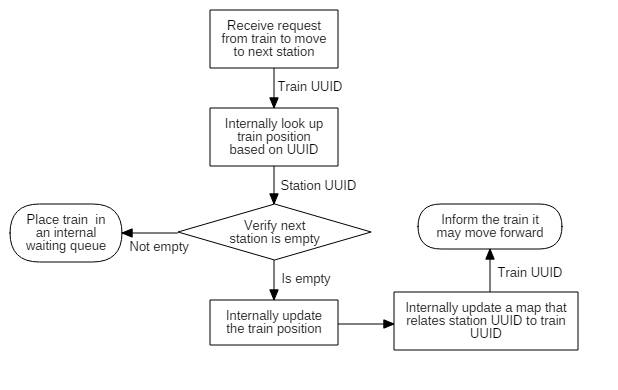
\includegraphics[width=5.5in]{moveToStation.png}
	\caption{Scheduler Logic for Moving Train into Station}
	\label{fig:movetostation}
\end{figure}

This station-to-train association HashMap is used when the station provides passengers for the train. The station sends a list of passengers and its station UUID back to the scheduler.  The scheduler then uses the map to route the passengers to the appropriate train.  It does this by generating a new message for its ``Board Passengers'' output port and sends the list of passengers in the message with the correct train UUID, rather than with the station UUID that was sent to the scheduler with the passenger list.  These scheduler internal data structures eliminate the need for all trains to be coupled to all stations and track sections.  It is a simple bookkeeping exercise for the scheduler.  However, any time information or objects need to be passed between models, a DEVS atomic model with appropriate input and output ports are utilized.
%

\subsubsection{Scheduler Log File}
To store the train positions over time, rather than send each train position to a transducer, the scheduler writes to a log file each time a train is moved. This allows the train positions to be plotted with an external tool, in this case \textit{matplotlib}.  The log file contains three columns of data: the scheduler clock value, the train UUID, and the array index representing station the train is moving into or leaving.  Data is written whenever the scheduler is updating the train position.  By only writing station indices and not track indices, it is easier to represent the time stopped at a station.  Fig.~\ref{fig:sampletrajectories} is an example of the trajectories for six trains on a subway loop with six stops.  Each color represents one train.  The horizontal segments of the trajectories represent the time spent stopped at a station. A positive slope represents travel in one direction and a negative slope represents the return trip. The travel time between stations is fixed, so variations in slope are representative of trains that must wait to enter or leave stations.  Overlap between two or more trains at a stop would indicate the scheduler is not functioning properly and allowing collisions.   
%
\begin{figure}[htb]
	\centering
	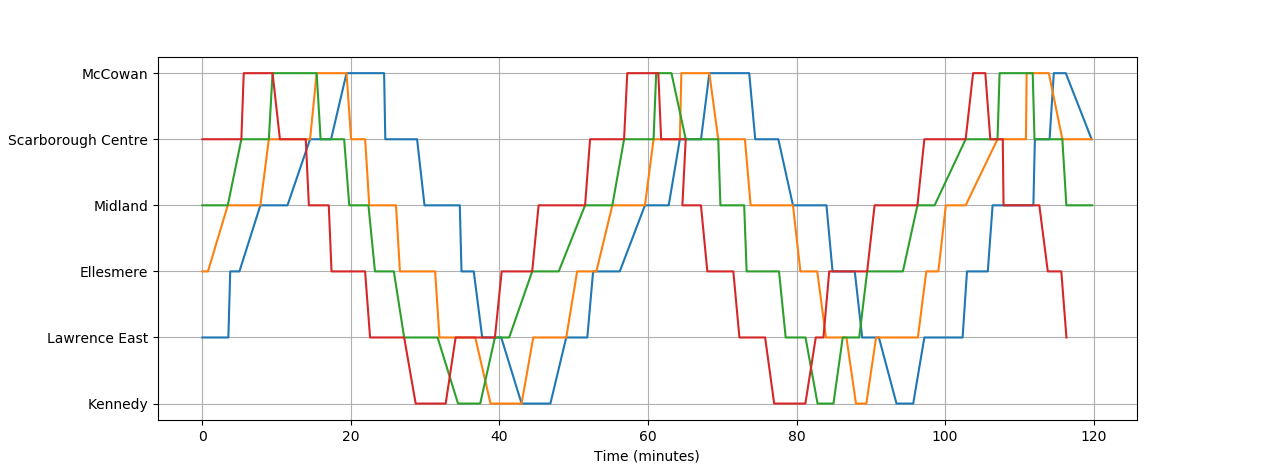
\includegraphics[width=7.0in]{sampletrajectories.png}
	\caption{Sample Trajectories from Scheduler Log File}
	\label{fig:sampletrajectories}
\end{figure}

\subsubsection{Scheduler Input Port Processing}
The scheduler processes all messages on all input ports before changing phase.  This all happens with zero time advance as all time advancement occurs in the train models.  In the external transition function, the model loops through all of the input ports and processes each of the messages on a given port.  When necessary, for example when a train has requested to move and the scheduler needs to respond, any output messages are generated and stored before the output function is called.  The output function then sends messages on all of the output ports at the same time.  This approach ensures that if multiple trains are arriving at different locations simultaneously, the scheduler is able to respond to each and every input it receives.  After all of the input ports have been processed, the scheduler then attempts to move each train in the waiting queue.

\subsection{Transducer Model}
The DEVS specification for the transducer model is given below.  The transducer model is used to collect some data about the entire subway system simulation and print some representative statistics. Each time a train provides passengers to the scheduler for unloading at a station, the scheduler will send the number of unloaded passengers to the transducer.  Since the stations produce passengers at a fixed rate, running various experiments over the same amount of time and examining the total number of passengers delivered to their destinations provides some insight on the total system passenger capacity.  If the system experiences significant delays, then the total number of passengers delivered is expected to go down.  Each train also maintains an internal clock to compute its own wait times. Every time the train is given a command to move by the scheduler, it provides its latest wait time to the transducer.  The transducer then provides a total sum of minutes waited by all trains in the system.  It also computes two averages.  The first average wait time uses all wait times provided, inclusive of zero values.  The second average wait time only uses non-zero wait times, meaning if and when there is a delay, this is the average of those delays.  Upon reaching the specified transducer observation time, it emits a stop signal to all of the trains that passivates them and ends the simulation.  Without this stop signal, the trains would run in perpetuity, making specific experimental observations difficult.
\begin{align*} DEVS_{\textrm{Transducer}} &= \left<X,Y,S,\delta_{ext},\delta_{int},\lambda,ta\right> \\
\Delta t &= \text{Observation Time} \\
X &= \lbrace (\text{``N Passengers Delivered''},(\mathbb{N}_0^+)), \\
 & (\text{``Wait Time''},(\mathbb{R}_0^+))\rbrace \\
Y &= \lbrace(\text{``Stop''},\lbrace True\rbrace)\rbrace \\
S &= \lbrace\text{``active'', ``passive''}\rbrace\times\Delta t \\
\delta_{ext}(\text{``active''},e,(\text{``N Passengers Delivered''},\mathbb{N}_0^+)) &= (\text{``active''},\sigma-e) \\
\delta_{ext}(\text{``active''},e,(\text{``Wait Time''},\mathbb{R}_0^+)) &= (\text{``active''},\sigma-e) \\
\delta_{int}(\text{``active''}) &= \text{``passive''} \\
\delta_{int}(\text{``passive''}) &= \text{``passive''} \\
\delta_{con}(s,ta(s),x) &= \delta_{ext}(\delta_{int}(s),0,x) \\
\lambda(\text{``active''}) &= (\text{``Stop''},True) \\
ta(s) &= \Delta t \\
ta(\text{``passive''}) &= \infty \\
\end{align*}

\subsection{Baseline Experimental Setup}\label{section:experiment_setup}
The Toronto Transit Commission (TTC) posts a large amount of data on the internet for their multiple forms of public transit.~\cite{ttcdata} Data available includes ridership, revenues, station usage, routes, and schedules.  Because the data available aids in choosing many quantities relative to this DEVS simulation, the TTC Scarborough Line is chosen as the basis for study.  Figure~\ref{fig:subwaymap} shows a map of this subway line.  It consists of six stations, is labeled line number three, and is colored blue.
%
\begin{figure}[htb]
	\centering
	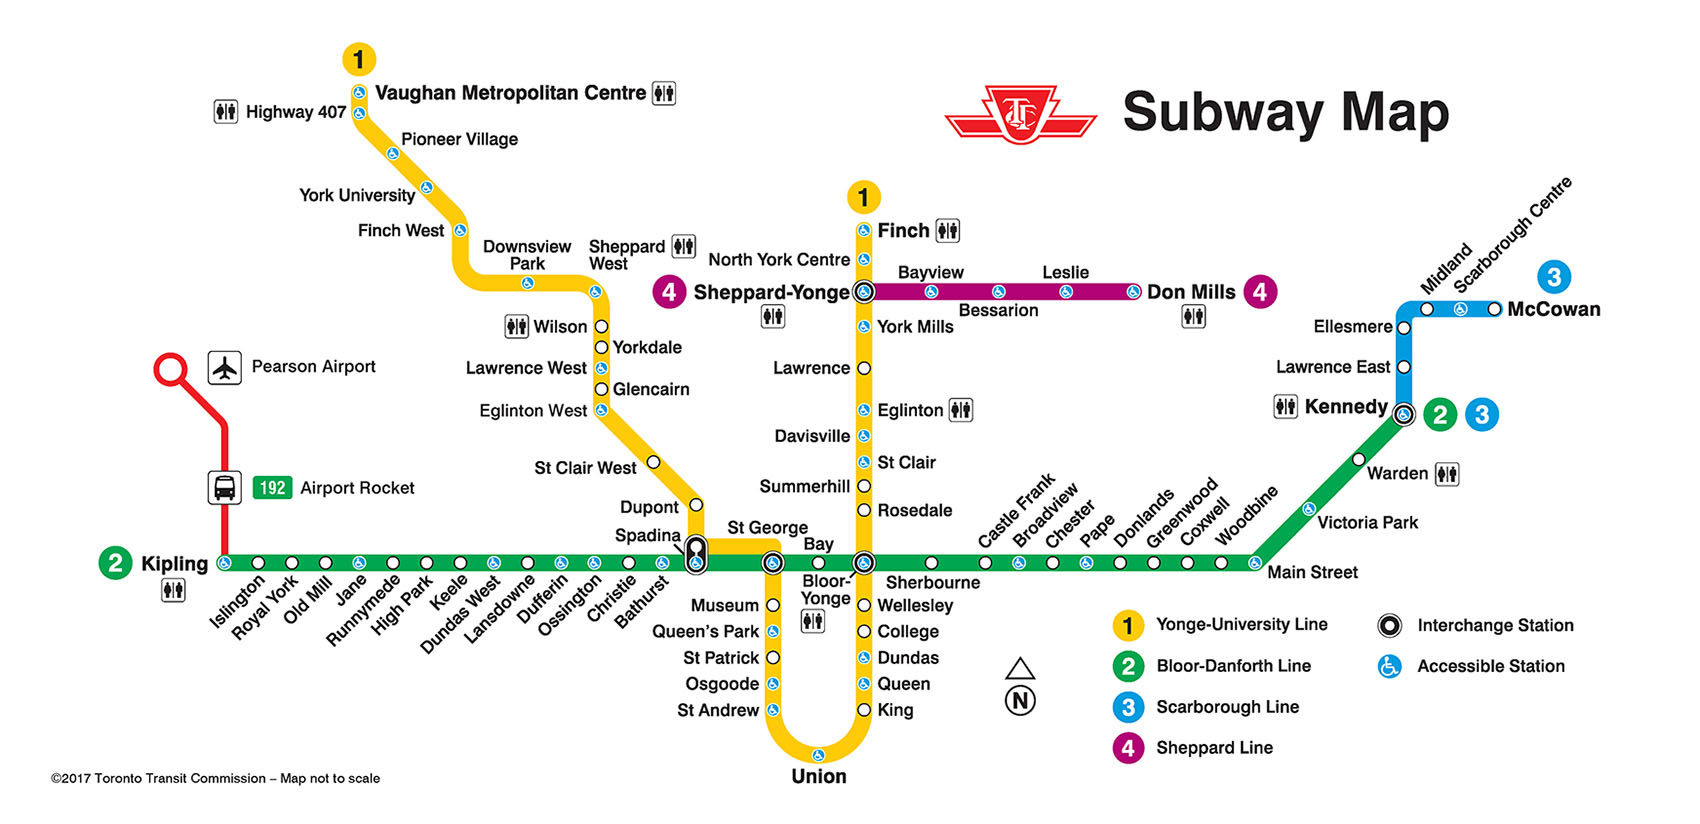
\includegraphics[width=7.0in]{SubwayFutureMap_lg.jpg}
	\caption{Toronto Subway System~\cite{ttcmap}}
	\label{fig:subwaymap}
\end{figure}
The Scarborough line as represented in this simulation is shown in Fig.~\ref{fig:scarborough}.  Each box in the figure represents a station instance, with one instance per direction per stop.  The arrows joining the stations represent the track sections and are labeled with the travel times between stations. As stored by the \texttt{SubwayLoop} class, the first item in the array is the Kennedy station instance and the last item in the array is the track section from Lawrence East (West) to Kennedy. The endpoints of the Scarborough line are modeled with single station instances, whereas all of the interior stations have instances for each direction of travel, as the station class effectively only models a single direction of travel.  The travel times between the stations are taken from the chart in Fig.~\ref{fig:traveltimes}.
%
\begin{figure}[htb]
	\centering
	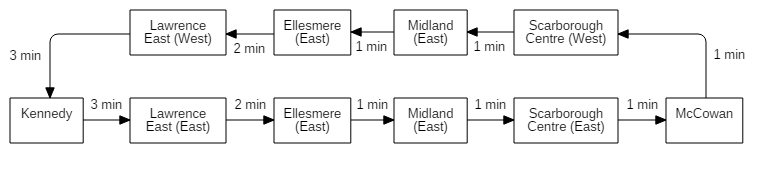
\includegraphics[width=7.0in]{ScarboroughLoop.png}
	\caption{Scarborough Loop Model}
	\label{fig:scarborough}
\end{figure}
%
\begin{figure}[htb]
	\centering
	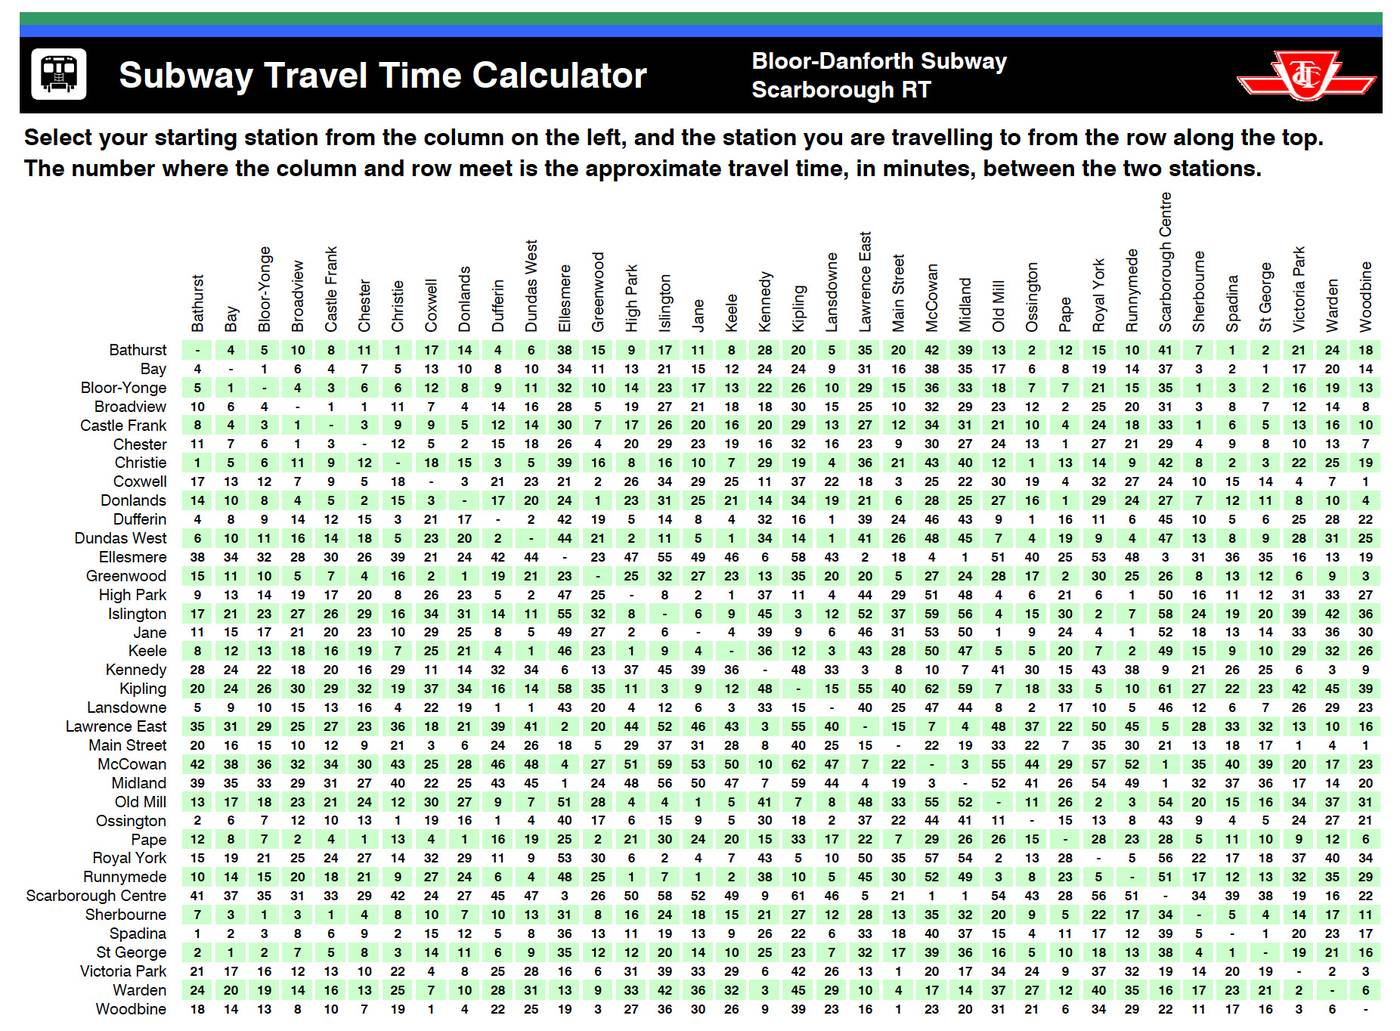
\includegraphics[width=7.0in]{ttc_travel_times_scarborough.jpg}
	\caption{TTC Travel Time Calculator~\cite{subwaytimes}}
	\label{fig:traveltimes}
\end{figure}

The most recent ridership data available for the Scarborough line is from 2015. Reference~\citen{ridershipdata} provides the number of passengers leaving and arriving at each station on an average business day.  For the Scarborough line, these values are provided in Table~\ref{table:ridership}.  To get the passenger generation rates, the average daily passengers to the trains are assumed over a twelve hour period.  So dividing the daily passengers by the number of minutes in an hour gives an initial rate.  Some of the stops are actually modeled with two station instances (one for each direction), so half the initial rate needs to be applied to each direction.  In some cases, half is not an integer value, so it is rounded up to the nearest integer.  This results in more passengers generated relative to the available data, but this is good as it can be considered more of a rush hour or stress case.
%
\begin{table}[htb]
	\centering
	\begin{tabular}{c|c|c}
		\textbf{Station} & \textbf{Average Daily} & \textbf{Applied Passenger Generation} \\
		                 & \textbf{Passengers to Train} & \textbf{Rate (Passengers/minute)} \\
		\hline\hline
		Kennedy & 17,969 & 13 \\
		Lawrence East & 4,326 & 4 \\
		Ellesmere & 864 & 2 \\
		Midland & 1,358 & 2 \\
		Scarborough Centre & 10979 & 8 \\
		McCowan & 2,857 & 4 \\
	\end{tabular}
\caption{Scarborough Line Ridership Details~\cite{ridershipdata}}
\label{table:ridership}
\end{table}

Reference~\citen{trainCapacity} offers some insight on the baseline train configuration for the Scarborough line.  The trains are known as the S-series trains and have a capacity of 30 seated and 55 standing passengers per train.  Currently, there are 6 four-car trains operating on the Scarborough line.

%The primary experiments will focus on disruptions in service due to train maintenance issues.  Given a train breakdown that causes a blockage on one of the tracks, we shall examine the effectiveness of a meet and pass routine.  Effectiveness shall be judged by the ability of the trains to pass by switching tracks without causing a deadlock, without causing significant delays in trains traveling in the opposite direction due to the track switching, and by monitoring passenger counts at the stations.  Monitoring the passenger counts is to evaluate that the service disruption does not cause a severe sustained surge in passengers waiting to board.  Another experiment will look at the effect of passenger surges at a given station, during rush hour for example, and the subway network's ability to maintain train movement given the increased loading and unloading times due to the surge. 

%These experiments will also involve varying the number of trains in service, with the goal of finding the optimum number of trains particular to the subway circuit modeled.  An increase in the number of trains may nominally be able to carry a larger number of passengers, assuming the number of trains does not exceed the number of stations.  However, if a disruption occurs and a train is disabled, this can quickly lead to deadlock as there is no extra bandwidth in the rail system to allow the trains to switch and get around the disabled train because all stations are occupied at any given time.  Conversely, if there are too few trains operating it runs the risk of not having enough total capacity to carry the influx of passengers, even though it may be easier to overcome service disruptions.

\subsection{Expected Outcomes}

The subway simulation in this paper is designed to focus on two outcome variables: passenger wait times at stations and train delays. The expected outcome from this simulation is that increases in passing areas decreases train delays and a increased number of trains to service a subway line results in lower passenger wait times at stations.


